\documentclass[12pt]{article}

\usepackage{graphicx} % Required for inserting images
\usepackage{setspace} % Required for paragraph setting
\usepackage{amsmath}

\usepackage{float} %H specifier in table

\usepackage[]{geometry}
% Set the page margins
\geometry{
    left=2.3cm,
    right=2.3cm,
    top=3cm,
    bottom=3cm,
}


\setlength{\parindent}{0pt}
\title{DESCRIPTIVE STATISTICS}
\author{Dr Kaombe}
\begin{document}
%
\maketitle
\newpage
\tableofcontents

\newpage

\section{Introduction}
\setlength{\parskip}{0.5em} % Set the desired paragraph spacing
\setstretch{1.5} % Set the desired line height between paragraphs
def 1: \textbf{Statistics} is the science of theory and methods of collection, organisation, analysis and interpretation of data sets so as to dertermine their essential characteristics.

There are established theories and approaches under each of the stages of data collection, organisation, analysis, interpretation and dissermination. These theories form a field of study called \underline{statistics}.

For instance underlying the stage of analysis of data is the vast mathematical apparatus of abstract concepts, theories, formulae, algorithm and so on that constitute the statistical tools that are employed to study a data set.

The tools allow an analyst to to build a framework for good decision making.
\newline
def 2: \textbf{Statistics} are mathematical quantities or expressions that are applied on data in order to elicit essential characteristics of the data at hand e.g the statistic for obtaining central value of the sample on the mean given by $\bar{x} = \frac{1}{n}\sum_{i = 1}^{n} x_i$ where $i = 1,2,3,4, \dots,19$ are sample parts.

def 3: \textbf{Statistics} may also imply the value calculated in def 2.
The third definition is ussually less found or used in formal context.

%end of section

\section{Types of statistics}
\subsection{Descriptive statistics}
Includes any treatment of data designed to summarize their essential features.

Interest is in arranging data in readable form eg using tables, charts and graphs or compute percentage, average, rate of change, variance, etc.

The aim of such task is to understand the data at hand and not beyond.

\subsection{Inferential or inductive statistics}is concerned with making estimates, predictions or forecasts and generalization.

It is  a process of infering something about the whole from an examination of only a part.

This process is carried out through sampling ie. using representative subgroup of items and conclude about the entire group/ population

Because conclusions are made by using information from a sample of items not every item, there is some level of error that will most assuredly taint the whole conclusions about the whole items.

Hence a measure of uncertainity of the surface made most accompanying in generalization.

%end of section

\section{Scales of Measurement}

\subsection{Norminal Scale}
It is associated with the word "name" and it identifies categories of data.

observations on the norminal scale posses neither numerical values nor order.
During data ananlysis numerical codes eg $0, 1, 2, 3$ can be assigned to outcomes of the measurement just for identification of category.

Example: sex variable whose outcomes are male or female is a variable on a norminal scale.
When numbers are used to classfy categories or levels of a variable that is on norminal scale, the magnitude of the differencies between those numerical values is meaningless.

This scale of measurement apply to qaulitative type of data or categorical data.

The only valid operations for variables represented by norinal scale are "$=$" or "$\neq$".
\subsection{Ordinal Scale}
It includes all the properties of norminal scale with additinal that the observations can be ranked from the smallest to the highest from the least important to the most important.

Example, type of car (Salon, Lorry, Bus).
Although the level of car is better than the other the ranking cannot indicate how much better, the numerical values assigned to data points just indicate type/ level of a car inorder of engine performance and the difference between the numerical values are meanings Eg. Type of membership to club:
\begin{enumerate}
    \item Ordinary member
    \item regular member
    \item Executive member
\end{enumerate}
Both norminal and ordinal scales are termed onmetric scales because the differences among their values are of no consequeces.
\subsection{Interval Scale}
It includes all properties of ordinal scale with additional property that the distance between the observations is meaningful.

The numbers assigned to the observations indicates order and posses the property that the difference between any two consecutive values is the same as the difference between any two other values (ie teh difference $10 - 9 = 1$ has the same meaning as $3 - 2 = 1$)

While this scale has a zero point, its location is arbitrary.

The ratios of interval scale have no meaning.
Eg: Temperature is measured on an interval scale. $0^{\circ}C$ does not imply the absence of heat. Alsp $40^{\circ}C$ is not twice as cold as $20^{\circ}C$

Grades of students in Mathematics is also an example of interval scale variable. A score of $0\%$ does not imply lack of knowledge.

The mathematical operations for handling variables measured measured on an interval scale are "$=$", "$\neq$","$>$","$<$","$+$","$-$".
\subsection{Ratio Scale}
Includes all the properties of interval scale with an added property that ratios of observations are meaningful. This is the case because absolute zero is uniquely defined.

Eg height of a person $0cm$ means the absence of any height and height of $8cm$ is twice as tall as height of $4cm$ (the ratio $\frac{8}{4} = 2$)

mathematical operations permitted under this scale are :

"$=$", "$\neq$","$>$","$<$","$+$","$-$", "$\times$", "$\div$"

Both Interval and ratio scales are callled metric scales (since the difference between values are meaningful)

Variables of these scales are quantitative.

%end of section

\section{Measures of Position}

\subsection{Percentiles}
The $P_{th}$ percentile of a group of numbers is that value below which lies $P\%$ (P percent) of the numbers in the group.

The Position of the $P_{th}$ percentile is given by
\begin{equation}
    P_{th} = \frac{(n+1)p}{100}
\end{equation}

When $n$ is the number of data points.

Example:

A department store's data on sales made by each  of its sales person. The data, number of sales made on a given data by each of $20$ sales persons are as follows
\begin{table}[H]
    \centering
    \caption{Data on sales}
    \begin{tabular}{|*{20}{c|}}

        \hline
        9  & 6  & 12 & 10 & 13 & 15 & 16 & 14 & 14 & 16 &
        17 & 16 & 24 & 21 & 22 & 18 & 19 & 18 & 20 & 17   \\
        \hline
    \end{tabular}
\end{table}


Find the $50_{th}$, $80_{th}$ and $90_{th}$ percentiles of this data set.

Solution:
\begin{table}[H]
    \centering
    \caption{Data on sales Sorted}
    \begin{tabular}{|*{20}{c|}}

        \hline
        6 & 9 & 10 & 12 & 13 & 14 & 14 & 15 & 16 & 16 & 16 & 17 & 17 & 18 & 18 & 19 & 20 & 21 & 22 & 24 \\
        \hline
    \end{tabular}
\end{table}

$n = 20$

\begin{enumerate}
    \item[(a)]50th Percentile \\ $P_{th}$ percentile $= \frac{(n + 1)p}{100}$
    $therefore$ $50_{th}$ $= \frac{(20 + 1)50}{100}$
    $= 10.5$

    The value at position $10.5$ is the same as the value at the middle of positions $10$ and $11$, which is the average of $16$ and $16$

    -Hence $50_{th}$ percentile is $16$

    Interpretation: This implies that $50\%$ of the given data points are below the value.
    \item[(b)] 80th Percentile
\end{enumerate}

\subsection{Quartiles}
Quartiles are the percentage points that break down the dataset into quarters.

First quarter, Second quarter, third quarter and fourth quarter

The first Quartile is the 25th percentile. It is tehe point below whil=ch lie one-fourth of the data.

Similary, the second quarterile is the 50th percentile. This is the most important pont and has a special name , it is the \textbf{median}

Definition: The median is a point below which lie half the data. it is the 50th percentile.

The third quartile is the 75th percentile point, it is that point below which lie $70\%$ of the data.

NB: 25th percentile is called lower qaurtile, 50th percentile is called the middle quartile. 75th percentile is called the upper quartile.

Example:

\subsection{Inter-Quartile Range (IQR)}
Definition: An interquartile range (IRQ) is the difference between the first and third quartiles.

The interquartile range is a measure of spread of the data.

IQR tells you the spread of the middle half of your distribution.

IQR contains the {difference between} second and third quartiles  or the middle half that data

IQR can be used to find outliers in data.

\subsection{Outlier analysis}

Outlier observations are the ones that do not confirm to distribution structure of the rest of the data.

The outliers can be identified by the following formulae:

\begin{equation}
    < Q_1 - 1.5\text{IQR or} > Q_3 + 1.5\text{IQR}
\end{equation}

%end of section

\section{Measures of Central Tendancy}

\subsection{Median}
\subsection{Mode}
\subsection{Mean}

\begin{equation}
    \bar{x} = \frac{\sum_{i = 1}^{n} x_i}{n}= \frac{x_1 + x_2 + x_3 + \ldots + x_n}{n}
\end{equation}


\begin{equation}
    \mu = \frac{\sum_{i = 1}^{N} x_i}{N}= \frac{x_1 + x_2 + x_3 + \ldots + x_N}{N}
\end{equation}


%end of section

\section{Measures of Variability / Dispersion}
The variance, range and interquartile range are some of the measurement of dispersion of a dataset.

They quantify amount of spread of data from the central value.
\subsection{Range}
NOT AVAILABLE
\subsection{Inter-Quartile Range (IQR)}
AVAILABLE IN UPPER SCTION
\subsection{Variance}
Sample variance of $X$ is
\begin{equation}
    S^2 = \frac{\sum_{i = 1}^{n}(x_i - \bar{x})^2}{n - 1} = \frac{\sum_{i = 1}^{n} x_i^2 - \frac{(\sum_{i = 1}^{n}x_i)^2}{n}}{n-1}
\end{equation}

It is average squared deviations of observations from the mean.

The square root of variance is called starndard deviatio, its symbol is $\delta$ for population data and $s$ for sample data

\begin{equation}
    S_x = \sqrt[2]{\frac{\sum_{i = 1}^{n} x_i^2 - \frac{(\sum_{i = 1}^{n}x_i)^2}{n}}{n-1}}
\end{equation}
\begin{equation}
    \delta = \sqrt[2]{\delta^2} = \sqrt[2]{\frac{\sum_{i = 1}^{N} x_i^2 - \frac{(\sum_{i = 1}^{N}x_i)^2}{N}}{N}}
\end{equation}

The standard deviation measures standard distance of each data point from their mean.
\subsection{Relative Variance and Coefiecient of Variation}

Relative variance is the ratio of variance of the data to the square of the mean of the data set. ie,
\begin{center}
    for sample mean
\end{center}
\begin{equation}
    V_{\bar{x}}^2 = \frac{S_x^2}{(\bar{X}^2)}
\end{equation}
\begin{center}
    OR
\end{center}
\begin{center}
    For population
\end{center}
\begin{equation}
    V_{\mu}^2 = \frac{\delta_x^2}{(\mu_x^2)}
\end{equation}

It is mostly used to compare variation across data sets, as $V_{\mu}^2$ or $V_{\bar{x}}^2$ has no units.

The square root of relative variance is called the coeficient of variation(Cv) or "relative error" of mean $\bar{x}$ or $\mu$

It is also dimensionless quantity and ussually given in percentages.

\begin{center}
    for sample mean
\end{center}
\begin{equation}
    CV_{\bar{x}} = \frac{S_x}{\bar{X}}
\end{equation}
\begin{center}
    OR
\end{center}
\begin{center}
    For population
\end{center}
\begin{equation}
    CV_{\mu} = \frac{\delta_x}{\mu_x}
\end{equation}


Eg: Given the sample data 1,2,3,4,5. Compute mean, variance, standard deviation, relative variance and coeficient of variation(CV)for the data.

Solution:

\begin{enumerate}
    \item[(a)] place holder for a
    \item[(b)] place holder for b
    \item[(c)] place holder for c
    \item[(d)] place holder for d
    \item[(e)] place holder for e
\end{enumerate}
\subsection{Recursion formulae for sample mean and variance}
- We can compute mean of $(n + 1)$ data poinsts effectively from knowing the mean ($\bar{x}$) of the first $n$ of them through a recursion formula for mean.
- Suppose we know $\bar{x}_{n}$ (ie average of $x_1, x_2, x_3, \dots, x_n$) and another observation $x_{n+1}$ becomes available then;

\begin{equation}
    x_{n + 1} = \frac{x_{n+1} + n\bar{x}_n}{n + 1}
\end{equation}

ie, the result for $(n + 1)^{st}$ term is obtained from the value of the $n^{th}$ terms.
eg. suppose the mean of a set of $n = 50$ values of some variable $x$ in $\bar{x}_n = \bar{x}_{50} = 63.75$. Let us now assume that a fifty-first obe=servation $x_{n + 1} = x_{61} = 22$ becomes available. What is the average of all data points?

solution



\begin{center}
    \[\bar{x}_{n + 1} = \frac{x_{n+1} + n\bar{x}_n}{n + 1}\]
    \[= \frac{22 + 50(63.75)}{50 + 1}\]
    \[= \frac{3209.5}{51}\]
    \[= 62.93\]
\end{center}


%end of section

\section{Measures of Symmetry}
\subsection{Skewness}
\textbf{Definition} An absolute frequency distribution is said to be skewed if it lacks symmetry.
- In other words, coeficient of skewness is a measure of symmetry of the distribution of a random variable.
- Skewness of data is measured by the pearsonian coeficient of skewness given by
\begin{equation}
    SK_p = \frac{\mu - mode}{\delta}
\end{equation}
- If the mode cannot be readily determined then we may employ a relationship among the mean, median and mode, given by
\begin{equation}
    \mu - mode = 3(\mu - median)
\end{equation}
to obtain
\begin{equation}
    SK_p = \frac{3(\mu - median)}{\delta}
\end{equation}
- For sample data, we can use $SK_p = \frac{3(\mu - median)}{\delta}$

- When $SK_p = 0$, it means $X_s^{'}$ absolute frequency distribution is symetrical aboute the mean
- when $SK_p > 0$ it implies that the distribution of $X$ is skewed to the right ie. It has a longer tail on the right hand side of mean.
- when $SK_p < 0$ it means that the distribution of $X$ is skewed to the left ie. It has a longer tail on the left hand side of mean compared to the right.

\hbox{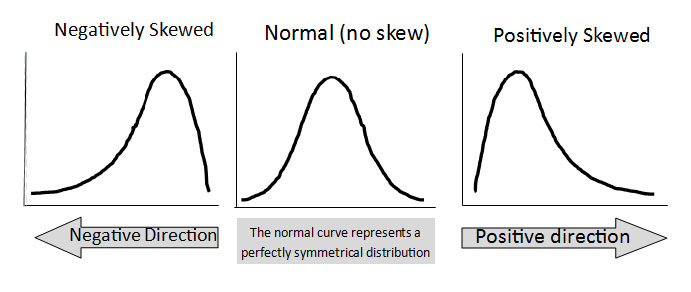
\includegraphics[width=\textwidth]{measure-of-skewness.jpg}}
- An alternative formula for computing skewness is through Quartiles. The Bowley's Coefiecient of skewness is given by
\begin{equation}
    SK_b = \frac{(Q_3 - Q_2)-(Q_2 - Q_1)}{Q_3 - Q_1}
\end{equation}
if $Q_2 - Q_1 = Q_3 - Q_2$, then the distribution is symetrical.
- if $Q_2 - Q_1 > Q_3 - Q_2$, the distribution is negatively skewed or skewed to the left.
- if $Q_2 - Q_1 < Q_3 - Q_2$, the distribution of $X$ is skewed to the right or is positively skewed.
\subsection{Kurtosis}
- Kurtosis refers to how flat or sharp the peak of the absolute frequency distribution happens to be.
- Both quantities are independent if units or dimensionless.
- The coeficient of kurtosis is estimated by
\begin{equation}
    K = \frac{\frac{(Q_3 - Q_1)}{2} }{P_90 - P_10}
\end{equation}

where the numerator $QD = \frac{(Q_3 - Q_1)}{2}$ is called quartile deviation, which measures half the distance between the 1st and 3rd quartiles. While $P_90$ is $90^{th}$ percentile and $P_10$ is $10^{th}$ percentile.

\hbox{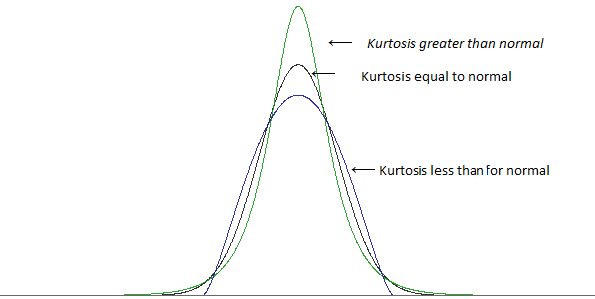
\includegraphics[width=\textwidth]{kurtosis.png}}

\end{document}
